\documentclass[12pt]{article}
\usepackage{graphicx}
\usepackage {color}
\usepackage{pdfpages}
\usepackage{float}
\usepackage{changebar}
\usepackage{enumitem,amssymb}
\renewcommand{\familydefault}{\sfdefault}
\usepackage[margin=1.2in]{geometry}
\usepackage{graphicx}
\usepackage{wrapfig}
\usepackage[super]{cite}
\usepackage{subcaption}
\usepackage[table]{xcolor}
\usepackage{amsmath}
\usepackage[sort, numbers]{natbib}
\usepackage{multirow}
\usepackage{tabularx}
\usepackage{siunitx}

%%%%%%%%%%%%Defining the margins %%%%%%%%%%%%%%%%%%%%%
\textheight 9.in
\textwidth 6.5in
\topmargin -.5in
\oddsidemargin 0in
\setlength{\parskip}{\smallskipamount}

%%%%%%%%%%%%%%Specific Commands %%%%%%%%%%%%%%%%%%
\newcommand{\eg}{{\em e.g.,}}
\newcommand{\ie}{{\em i.e.,}}
\newcommand{\etc}{{\em etc.,}}
\newcommand{\etal}{{\em et al.}}
\newcommand{\degrees}{{$^{\circ}$}}
\newcommand{\fig}[1]{Figure~\ref{#1}}
%%%%%%%%%%%%%%%%%%%%%%%%%%%% Setting to control figure placement
% These determine the rules used to place floating objects like figures 
% They are only guides, but read the manual to see the effect of each.
\renewcommand{\topfraction}{.9}
\renewcommand{\bottomfraction}{.9}
\renewcommand{\textfraction}{.1}
\renewcommand{\familydefault}{\sfdefault} %setting the san serif font

%%%%%%%%%%%%%%%%%%%%%%%% Line spacing
% Use the following command for ``double'' spacing
%\setlength{\baselineskip}{1.2\baselineskip}
% and this one for an acceptable NIH spacing of 6lpi based on 11pt
%\setlength{\baselineskip}{.9\baselineskip}
% The baselineskip does not appear to work when we include a maketitle
% command in the main file.  Something there must set the line spacing
% If we use this next command, then things seem to work.
\renewcommand{\baselinestretch}{.9}

\setcounter{secnumdepth}{0} %make no numbers but have a table of contents


\begin{document}

\title{Lab 4: ECG Sim}
\author{Jake Bergquist, u6010393 }
\maketitle

\section{Introduction}
\par{}
Simulation based on models for the electrical activity of the heart are becoming a more and more common approach for the study and understanding of the way in which electrical potentials propagate from the heart to the torso surface as well as for the study of the underlying cardiac electro-physiology.[|<cite brett and such>] From this research effort, investigative tools such as ECGSIM have been developed to better interrogate the relationships between simulated cardiac action potentials and the resultant cardiac and torso electrical activity. 

In this lab our goal was to utilize ECGSIM to investigate the relationship between the characteristics of the heart such as the simulated action potentials on the heart surface and the resultant electrograms as measured on the heart and torso surface. In particular we focused on visualizing features of the action potential reflected on the epicardial and torso ecgs. ECGSIM allows the user a wide array of available manipulations of the underlying cardiac sources as well as several modalities of visualization. Using ECGSIM we can manipulate the upstroke time, amplitude, plateau duration, repolarization time, and baseline membrane voltage. ECG sim then uses these parameters the alter an underlying action potential model and generate transmembrane, and extracellular potentials for a heart beat. These simulated values zare the mapped onto a heart geometry and propagated through a torso geometry to the torso surface. The user can choose to view a rich amount of data in the form of potential maps, activation times, recovery times, ARI, and ecg leads from various torso recording locations. The changes made to the action poitentials can be made locally with a varying radius of effect even allowing control of transmural, epicardial or endocardial modification.

We utilized ECGsim to assess several action potential characteristics, specifically upstroke time, plateau duration and repolarization time, and how these effected potential maps, ARI, activation maps, BSP measurements, and ECG measurements. We the examined how manipulations of the underlying action potential model result in alterations to these measured parameters. The exploration of this simulation tool allows for a better understanding not only of the relationships between cardiac action potentials across the heart and the resulting potential and other metric distributions. We also explore more generally the practical advantages and limitations provided by simulation tools and formulations such as ECGSIM.

\section{Methods}
\subsection{Question 1}
In order to investigate the relationships between the activation of the ventricles as shown by the activation map and the potential distributions on the cardiac surface I first visualized the activation map an noted an area of early activation. I then identified its activation time. I then looked at the potential map of the epicardium int he same location and investigated what happened to the potentials when I moved through the time point identified by the activation map. I also examined the relationship between the activation map and the time signals for the action potentials as well as the ECG leads. I then repeated this process with repolarization maps.

\subsection{Question 2}
To investigate the relationship between activation recovery interval (ARI) and action potential duration (APD) I eamined the ARI map. I then selected nodes with various ARI values and investigated the underlying action potentials. Finally I modified the repolarization time of the action potential and observed the effects on ARI.

\subsection{Question 3}
To explore the ability of ECGSIM to modify the simulated action potentials and their resulting projection to the torso I selected a region of the heart to modify. I then reduced the action potential duration in that region and observed the effect on activation, recovery, ARI, and body surface potentials. I focused on the change in body surface potentials and the resulting ECGs fromt he body surface between the baseline and the modified local action potentials.

\section{Results}
\subsection{Question 1}
In \fig{fig:ActT} the activation map is shown and specifically we are focused on a region of early epicardial activation. In \fig{fig:ActT_pot} I explored the potential distribution by panning through time and saw that as this section underwent the upstroke of the action potential a negative potential appeared int eh same region as the low activation time. Thus it seems that the activation time can be seen on the epicardium by a shift to a negative potential. Additionally as most of the heart had reach this activationt his corresponded to a time in the QRS of the body surface ECGs of a steep slope.
\begin{figure}[H]
	
	\centering
	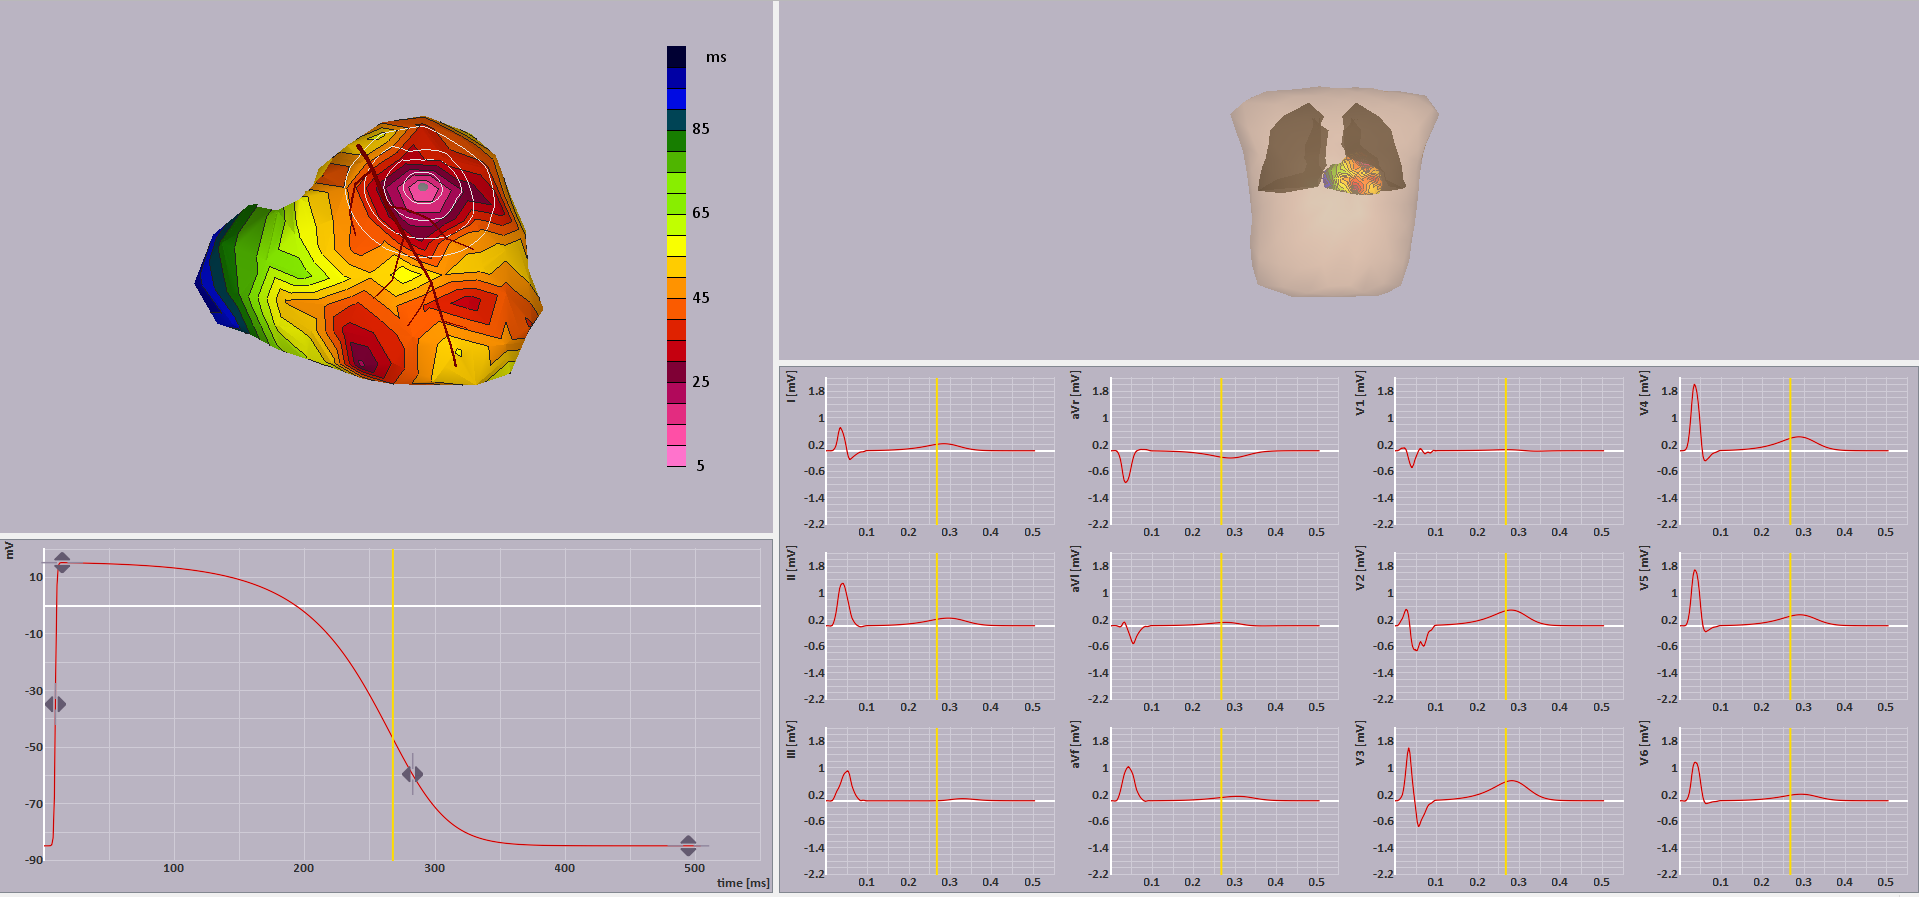
\includegraphics[width = .8\textwidth]{Figures/ActTimes.png}
	\caption{Activation map of epicardium. The area hilighted is one of early activation on the epicardium as depicted by the activation map.}
	\label{fig:ActT}
\end{figure}

\begin{figure}[H]
	
	\centering
	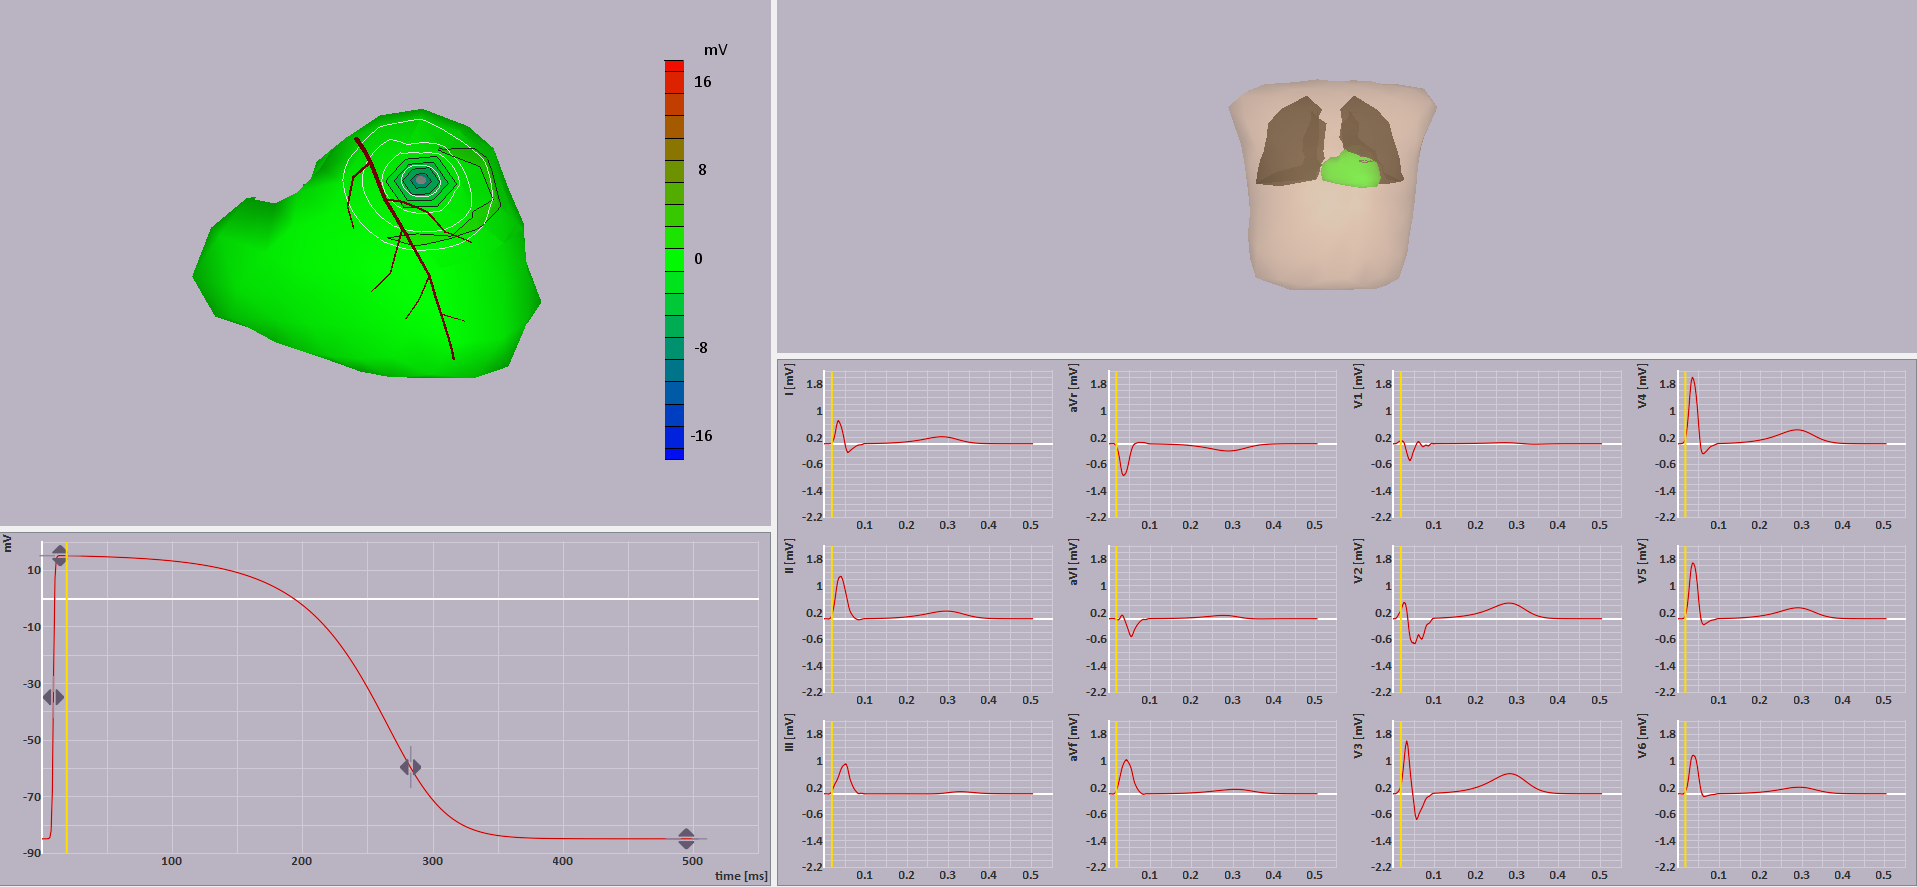
\includegraphics[width = .8\textwidth]{Figures/ActTimePotentials.png}
	\caption{Potential distribution during activation of the highlighted region. As can be seen there is a negative potential that develops at the site of activation when we scroll in time to that particular activation time for that region in the signal. }
	\label{fig:ActT_pot}
\end{figure}

In the case of repolarization, \fig{fig:RecT} shows the recovery map for the epicardium. As can be seen the recovery map is far less ordered. Again I focused on an area of early recovery. When I moved the time signal to roughly the indicated recovery time (260 seconds) I saw that the action potential was no longer in plateau and was roughly halfway through repolarization. This manifested as a positive potential on the epicardium as can be seen in \fig{fig:RecT_pot}.

From ym observations it seems that the presence of a potential that goes from positive or neutral to negative during the early parts of the signal identify the activation of that region of the heart. This corresponds to the upstroak of the action potential, and on the ECG this corresponds to the QRS (the activation of the ventricles occures during the QRS). Specifically the major downstroak fo the QRS identifys the activation time for that electrode overall. In the case of repolarization I saw that this occured during the T wave of the electrogram. This the T wave can be used to detect the recovery time for a given electrogram. An algorithm to detect activation and recovery would first look int eh QRS or the early part of the signal and find the greatest downward slope (greatest negative derivative) of the signal. To find the recovery time the algorithm would look in the T wave or the latter half of the beat and find the greatest positive slope, or the greatest positive derivative. Of course these methods are senesitive to noise, pacing artifacts and irregular beats. As such more comprehensive methods would utilize these and other metrics to confirm activation and recovery from electrograms.

\begin{figure}[H]
	
	\centering
	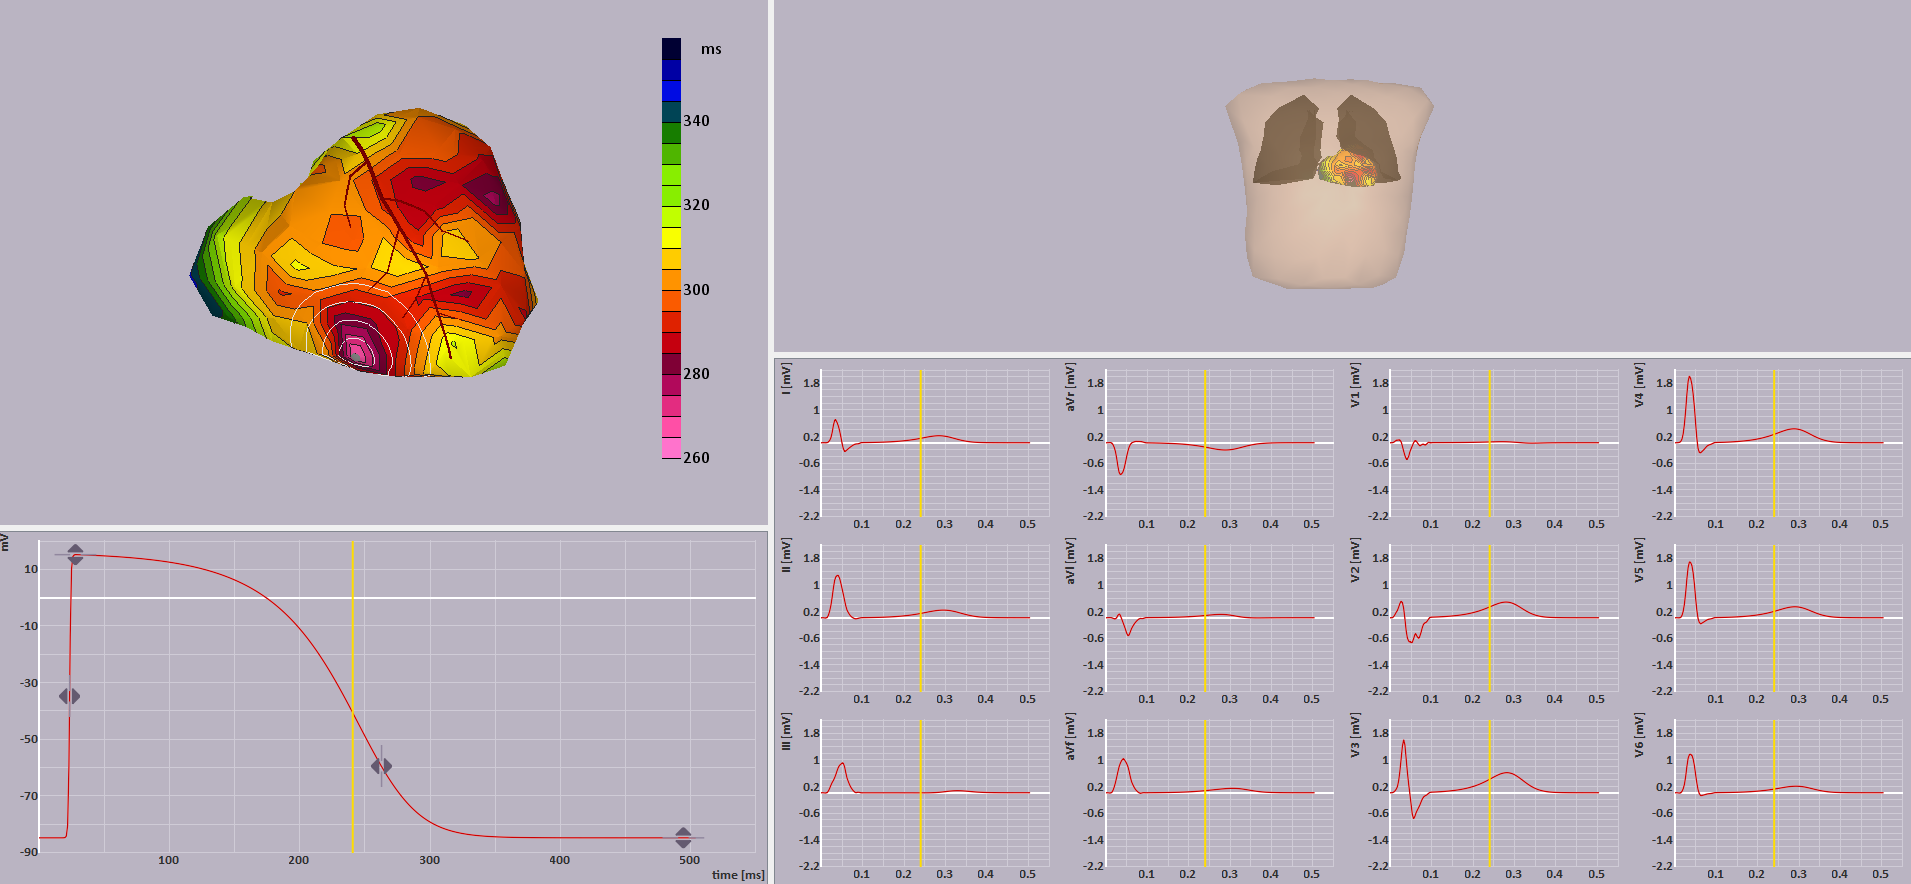
\includegraphics[width = .8\textwidth]{Figures/RecoTimes.png}
	\caption{Recovery map of epicardium. The area hilighted is one of early recovery on the epicardium as depicted by the recovery map.}
	\label{fig:RecT}
\end{figure}

\begin{figure}[H]
	
	\centering
	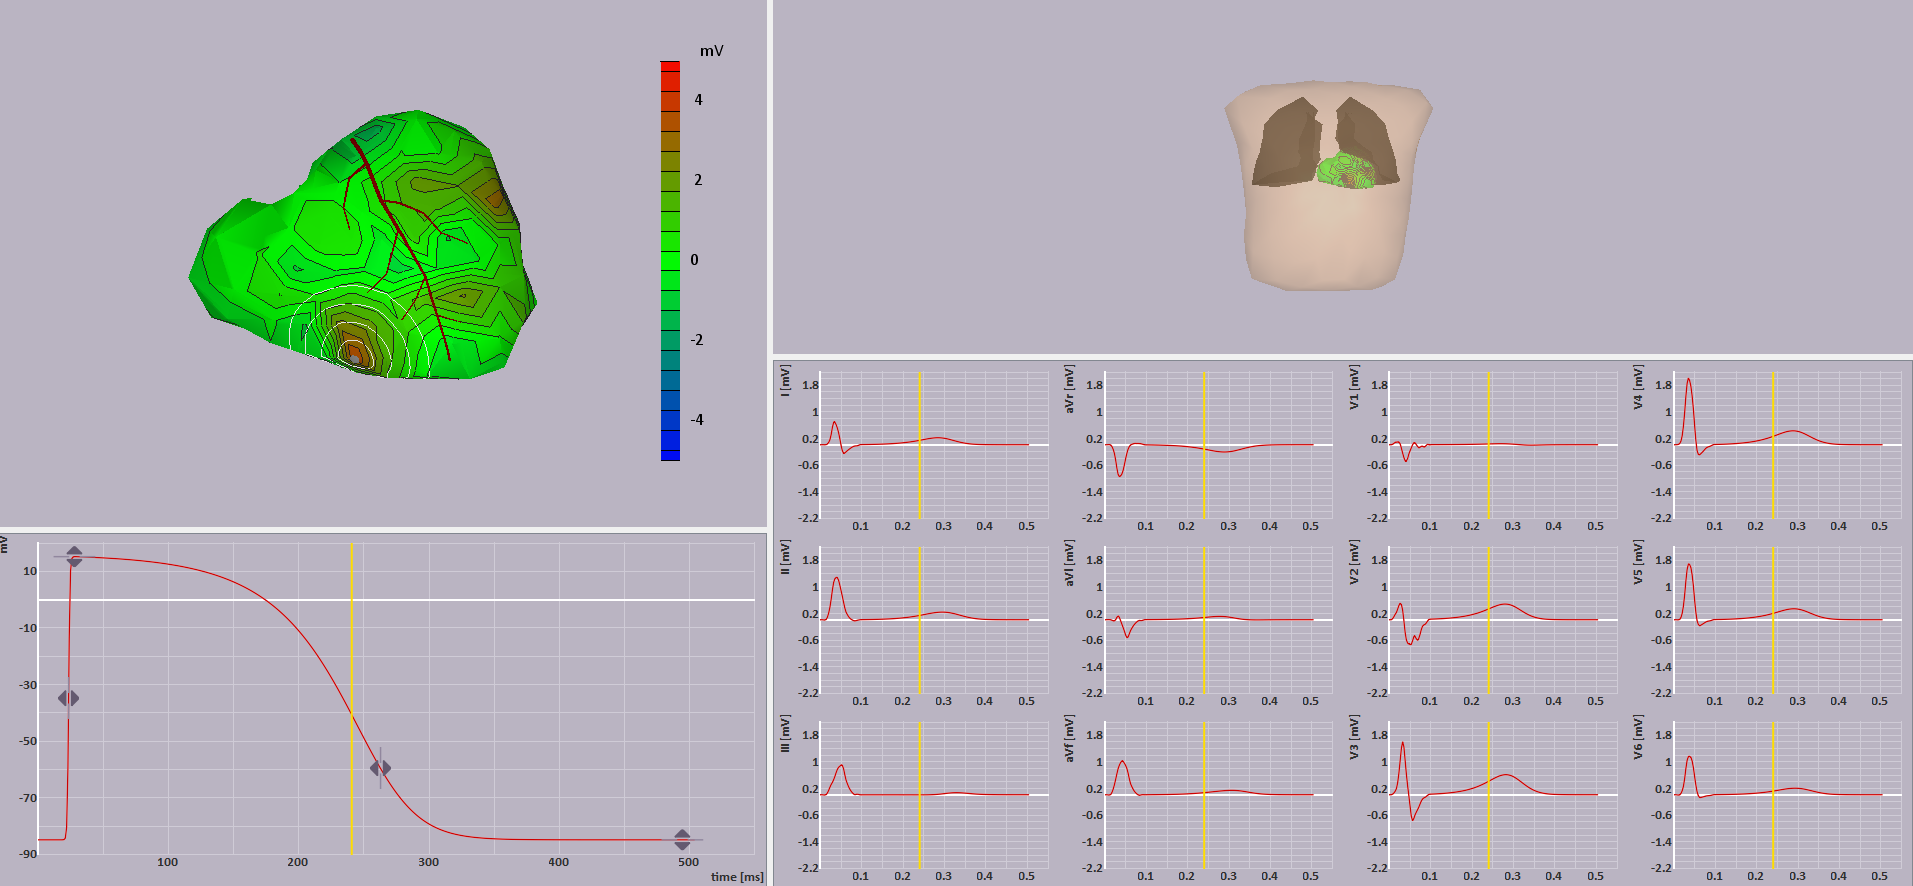
\includegraphics[width = .8\textwidth]{Figures/RecoPots.png}
	\caption{Potential distribution during recovery of the highlighted region. As can be seen there is a positive potential that develops at the site of activation when we scroll in time to that particular recovery time for that region in the signal.}
	\label{fig:RecT_pot}
\end{figure}

\subsection{Question 2}
To investigate the relationship between APD and ARI I displayed the ARI on the epicardium and endo cardium and investigated several areas. As can be seen in \fig{fig:APD} at each different instance the ARI value corresponds to the time between the upstroke (activation) and the repolarization (recovery) phases of the action potentials. This holds in different parts of the epicardium (\fig{APD:epi},\fig{APD:epi2}) and the endocardium (\fig{APD:endo}). Additionally when the recovery/repolarization is adjusted to be later, this results in a larger value of the ARI in that region of the heart (\fig{APD:epichanged}).

\begin{figure}[H]
	\centering
	\begin{subfigure}{0.45\textwidth}
		\centering
		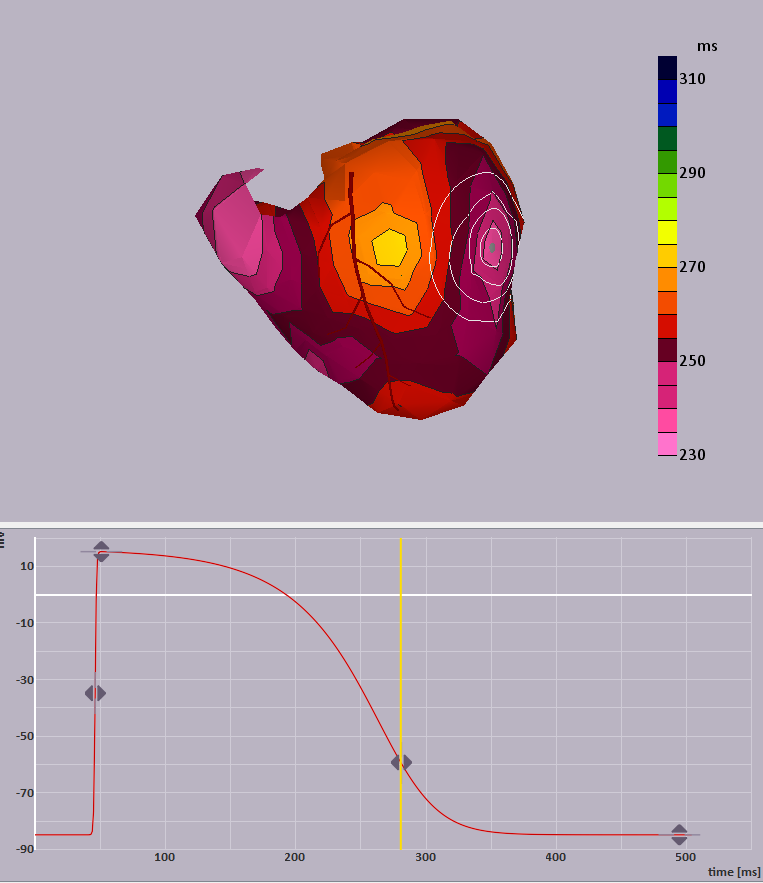
\includegraphics[width = \textwidth]{Figures/EpiADP.png}
		\caption{}
		\label{APD:epi}
	\end{subfigure}
	\begin{subfigure}{0.45\textwidth}
	\centering
	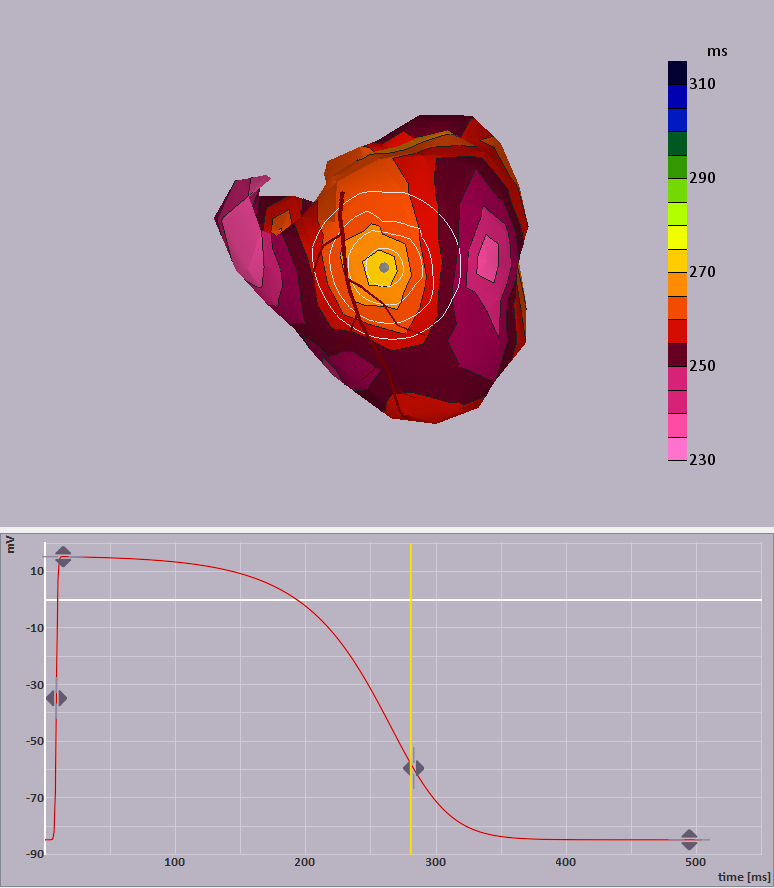
\includegraphics[width = \textwidth]{Figures/ADP_check1.png}
	\caption{}
	\label{APD:epi2}
	\end{subfigure}
	\begin{subfigure}{0.45\textwidth}
		\centering
		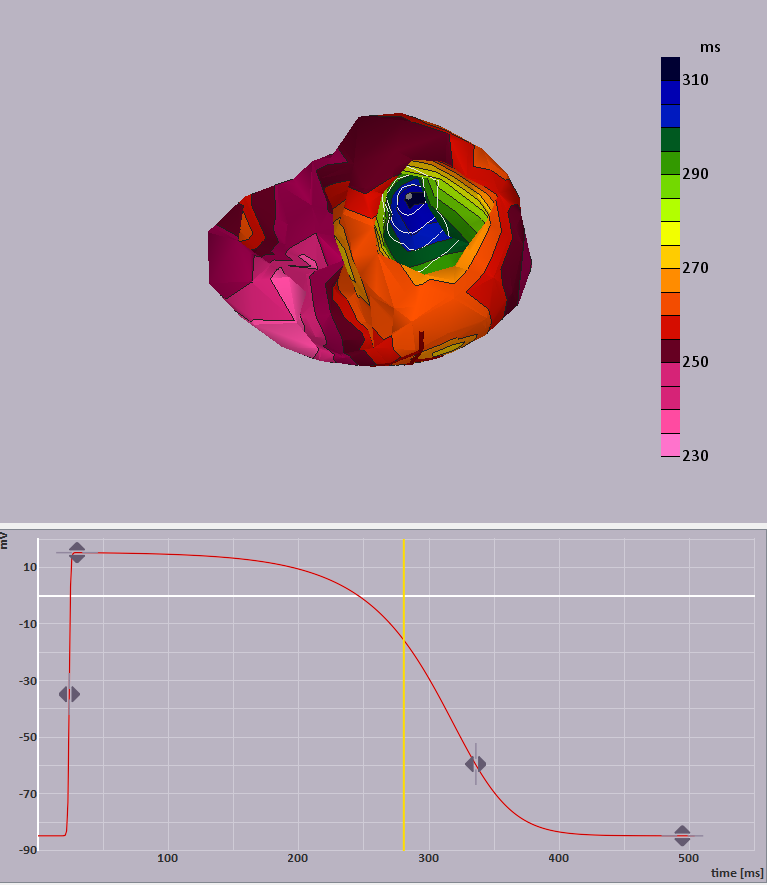
\includegraphics[width = \textwidth]{Figures/EndoADP.png}
		\caption{}
		\label{APD:endo}
	\end{subfigure}
	\begin{subfigure}{0.45\textwidth}
		\centering
		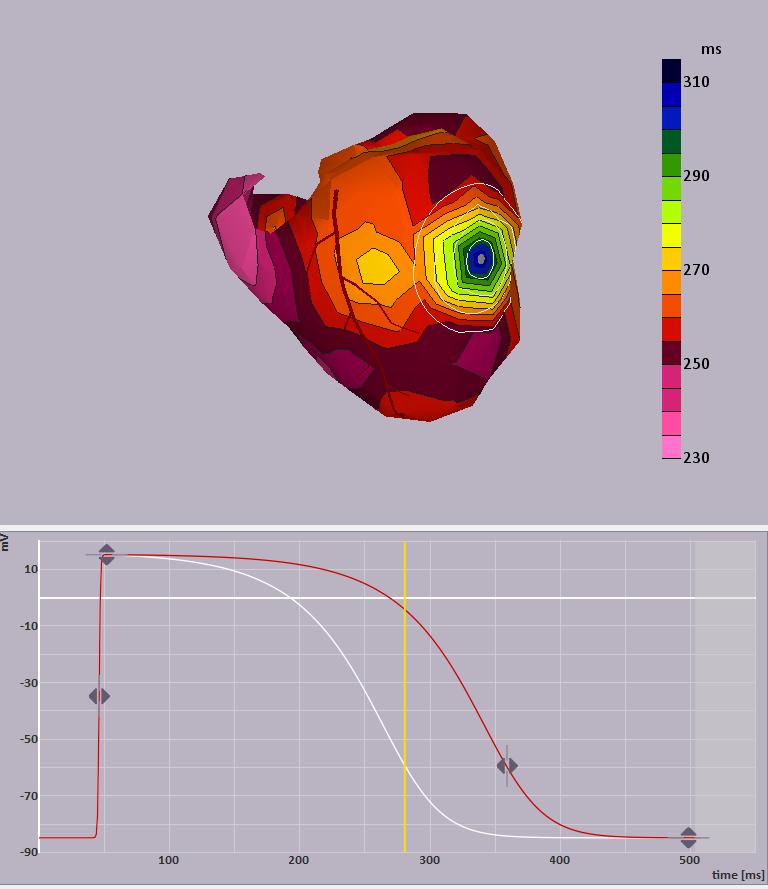
\includegraphics[width = \textwidth]{Figures/EpiChangedADP_1.png}
		\caption{}
		\label{APD:epichanged}
	\end{subfigure}

	\caption{Action potential duration and activation recovery interval for several locations. Two epicardial regions (a,b), and an endocardial region (c) are shown with default signals. A location on the epicardium was chosen and the action potential duration was increased. The resulting ARI map was shown(d). }
	\label{fig:APD}
\end{figure}

\subsection{Question 3}
I identified that the recovery time was an interesting part of the signal to change by affecting the duration of the action potential. By reducing the local action potential duration I could also reduce the local recovery time as seen in \fig{fig:BSP}. As recovery defines the T wave I looked to see the effect of this manipulation on the T wave Body surface potentials  (BSP). I saw that this change caused an increased positive potential on the BSP during the P wave in a region of the chest directly above the affected area of the heart. Additionally the ECG signals changed dramatically with respect to the T wave, particularly the precordial leads (V1-V6)(\fig{BSP:alt}).

\begin{figure}[H]
	\centering
	\begin{subfigure}{\textwidth}
		\centering
		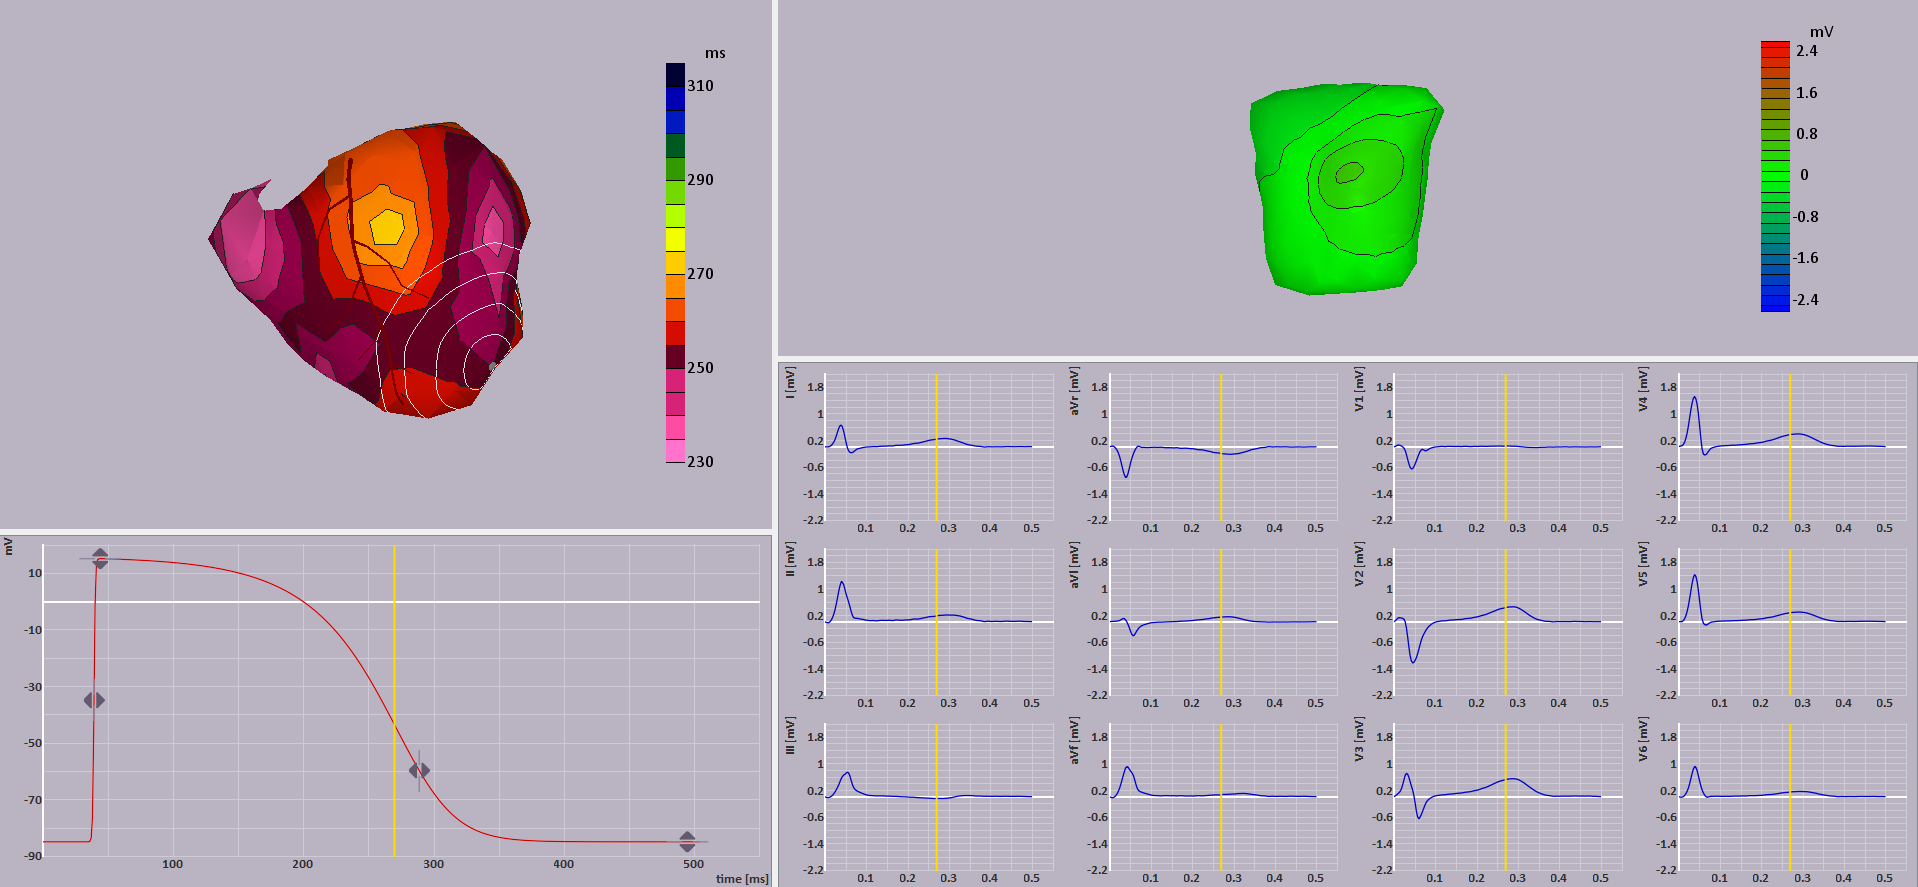
\includegraphics[width = \textwidth]{Figures/baselineBSO.png}
		\caption{}
		\label{BSP:Baseline}
	\end{subfigure}
	\begin{subfigure}{\textwidth}
		\centering
		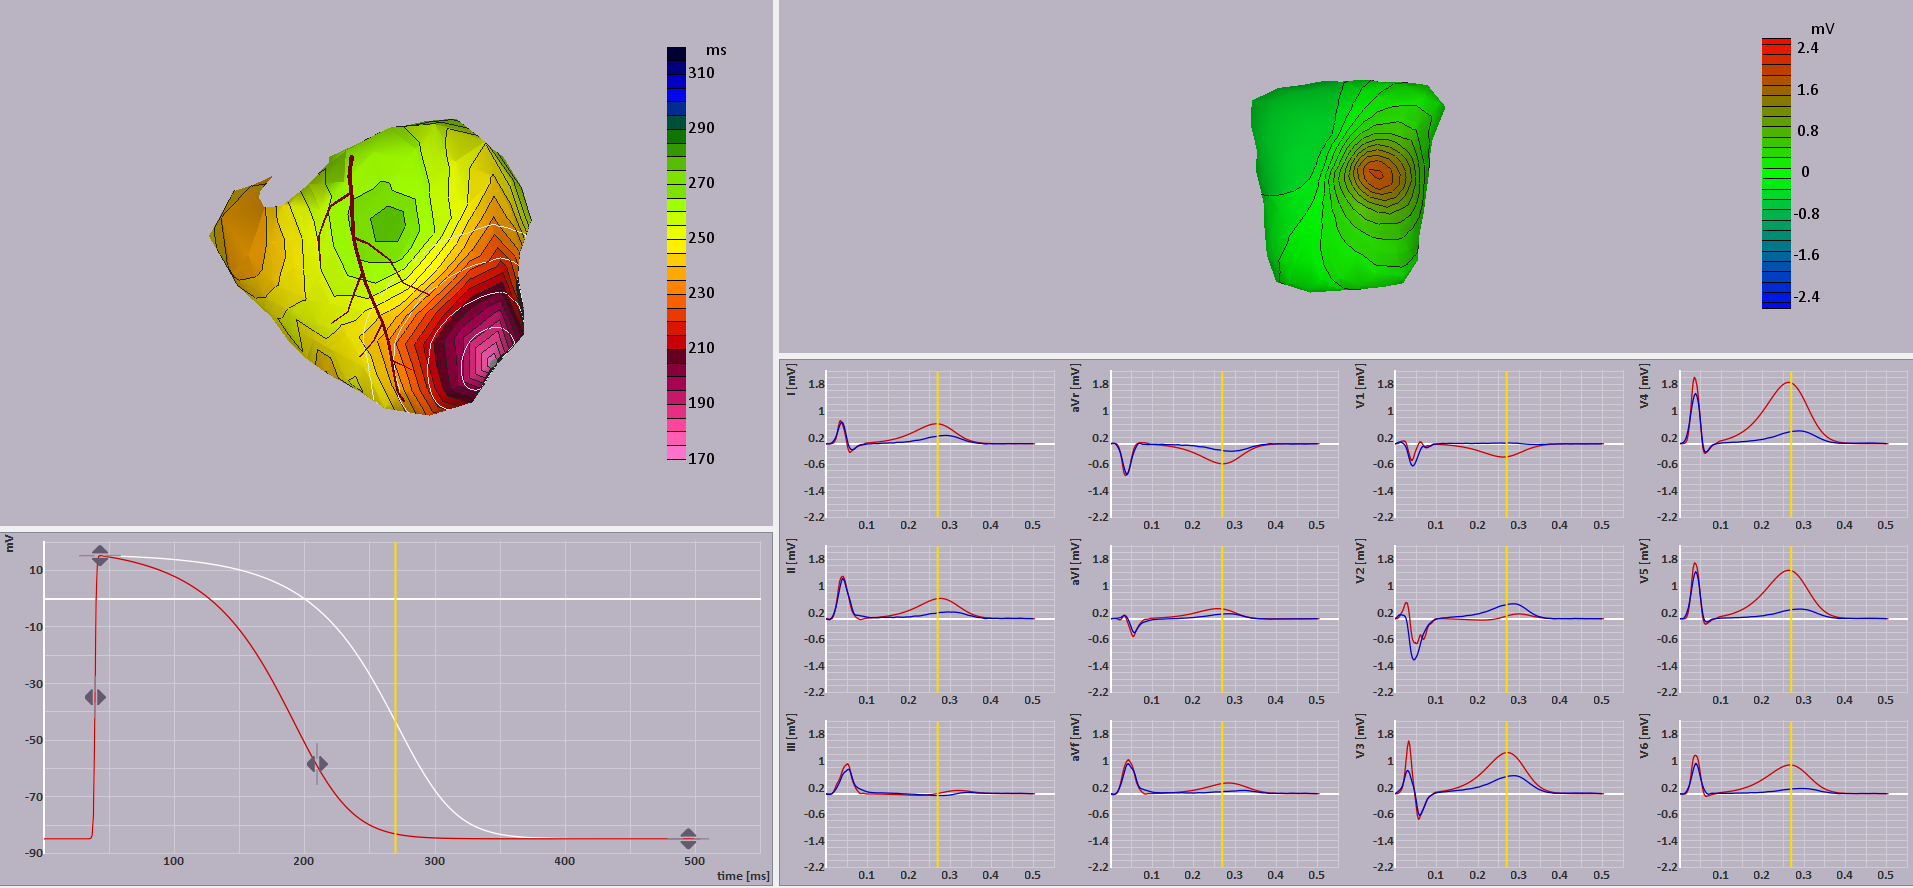
\includegraphics[width = \textwidth]{Figures/AltAPD_BSP.png}
		\caption{}
		\label{BSP:alt}
	\end{subfigure}

	
	\caption{}
	\label{fig:BSP}
\end{figure}

\section{Discussion}
During this lab I explored the used of ECGSIM to understand the relationship betweent he measured BSP and epi/endocardial potentials to the underlying action potentials that ultimatly generate these signals we measure. I found that changing parameters such as the activation time and recovery time has dramatic affects not only on the obvious activation and recovery times but also the potential distributions on the heart and the torso. The ability to directly manipulate these parameters in an unlimited way is a strength of simulation based exploration that is unrivaled by non simulated experimentation. The ability to immediately and quickly change any parameter of the hearts electrical functioning is unparalleled. Such access allows for the controlled examination of phenomena that would be impractival to investigate in live models. For example, atypical rhythms in the heart such as premature ventricular contractions are very commonly studied. However it can be challenging to interpret experimental findings regarding PVCs as natrual PVCs can originate in many places in the heart. to understand the resulting patterns observed on ecg or surface potentials one could use simulation to emulate PVCs across the heart and examine the resulting potential distributions.Overall the shear amount of data accessible and parameter modification available are not possible with experiments. However, simulations cannot allow for examination of situations they were not parameterized to capture. In general all models (such as those simulations are built from) are wrong in some way, but useful in some scenarios. Thus one must be careful when using simulations to ensure that the simulation is well posed to answer the desired questions. 
%%%%%%%%%%%%%%%%%% Correct Bibliography Style

%\bibliography{C:/Users/Jake/Documents/library}
%\bibliographystyle{IEEEtran}


\end{document}








